% Build with: latexmk -pdf main.tex
\documentclass[11pt]{article}

\usepackage[T1]{fontenc}
\usepackage{lmodern}
\usepackage[margin=1in]{geometry}
\usepackage{microtype}
\usepackage{amsmath,amssymb,amsthm,mathtools}
\usepackage{booktabs}
\usepackage{enumitem}
\usepackage{xcolor}
\usepackage{tikz}
\usetikzlibrary{calc}
\definecolor{fts}{RGB}{20,70,170}
\usepackage[colorlinks=true,linkcolor=blue!50!black,citecolor=blue!50!black,urlcolor=blue!50!black]{hyperref}

\theoremstyle{plain}
\newtheorem{theorem}{Theorem}[section]
\theoremstyle{definition}
\newtheorem{definition}[theorem]{Definition}

\newcommand{\bits}[1]{\{0,1\}^{#1}}
\newcommand{\getsr}{\stackrel{\$}{\gets}}
\newcommand{\Th}{\mathsf{Th}}
\newcommand{\Enc}{\mathsf{Enc}}
\newcommand{\Digest}{\mathsf{Digest}}
\newcommand{\Gen}{\mathsf{Gen}}
\newcommand{\Sig}{\mathsf{Sig}}
\newcommand{\Ver}{\mathsf{Ver}}
\newcommand{\hash}{\mathsf{H}}
\newcommand{\LE}{\mathsf{LE}}
\newcommand{\Truncate}{\mathsf{Truncate}}
\newcommand{\concat}{\mathbin\Vert}
\newcommand{\sk}{\mathit{sk}}
\newcommand{\pk}{\mathit{pk}}
\newcommand{\rootnode}{\mathit{root}}
\newcommand{\addr}{\mathsf{A}}
\newcommand{\amax}{A_{\max}}
\newcommand{\cmax}{C_{\max}}
\newcommand{\idx}{\mathit{idx}}
\newcommand{\lut}{\mathsf{code}}
\newcommand{\OtsSign}{\mathsf{Ots.sign}}
\newcommand{\OtsLeaf}{\mathsf{Ots.leaf}}
\newcommand{\TreeFold}{\mathsf{Tree.fold}}
\newcommand{\FtsKey}{\mathsf{Fts.key}}
\newcommand{\FtsOpen}{\mathsf{Fts.open}}
\newcommand{\FtsRec}{\mathsf{Fts.recover}}

\emergencystretch=1.5em
\setlist[enumerate]{leftmargin=2em, itemsep=4pt}

\title{leanSPHINCS}
\author{}
\date{}

\begin{document}
\maketitle

\begin{abstract}

This specification defines leanSPHINCS, a stateless hash-based signature scheme whose few-time signature is built from small WOTS keys and whose hash inputs are laid out in 16-byte words (Section~\ref{sec:layout}).

\begin{itemize}
  \item \textbf{NIST security level~1}~\cite{NISTPQC}, 127 bits of classical security in the Random Oracle model, and a target of $\approx 64$ bits in the Quantum Random Oracle model (Section~\ref{sec:security}).
  \item \textbf{Public key: 32 bytes.}
  \item \textbf{Signature: 4276 bytes.}
  \item \textbf{Verification: 307 compressions} of BLAKE2s.
  \item \textbf{Lifetime: up to 1.3B signatures per key pair}, less for a key that trades lifetime for a faster key generation (Section~\ref{sec:security}).
\end{itemize}
\end{abstract}

The scheme has the shape of SLH-DSA-128-24~\cite{SP800230}, a single Merkle tree of one-time keys, each signing one few-time key. The one-time signature is WOTS$^+$C~\cite{HK22C}. The few-time signature is not FORS but a two-level forest of small WOTS keys, an idea inspired by ~\cite{siggolf}. A key may be pruned~\cite{conduition}. The definitions below specify the scheme completely.

\section{Hashing and parameters}
\label{sec:parameters}

Write $\bits r$ for $r$-bit strings, $0^r$ for $r$ zero bits, $\concat$ for concatenation, $\LE_r(z)$ for the unsigned $r$-bit little-endian encoding of $z$, and $\LE^{-1}$ for its inverse. Write $x\getsr A$ for a uniform sample from $A$. Indices and bit positions start at zero; $\bot$ denotes failure.

Let $\hash:\bits{*}\to\bits{256}$ be BLAKE2s. Most operations use its first $n=128$ output bits:
\[
  \Th(P,\addr,M)=\Truncate_n\!\left(\hash(P\concat\addr\concat M)\right).
\]
Here $P$ is a 128-bit public parameter and $\addr$ is a 128-bit \emph{address} identifying the operation and its position in the construction. Appendix~\ref{sec:tweaks} gives every address's exact bytes. $\Truncate_r$ always keeps the first $r$ bits, with bits read least significant first within each byte. The parameter and the address take half of a block's 64 bytes, so a chain step and a Merkle node each cost one compression, and every value a hash input holds starts on a 16-byte boundary.

The message $m$, the seed $S_0$ and the secret $S$ derived from it are each 256 bits. The signature contains a 128-bit randomizer $\rho$ and one 32-bit counter $c$. Chain values and Merkle nodes are 128 bits; write $\mathcal H=\bits n$.

\begin{center}
\begin{tabular}{@{}lll@{}}
\toprule
Symbol & Value & Meaning\\
\midrule
$w$ & $2$ & bit-size of WOTS$^+$C chain positions\\
$v$ & $64$ & chains per WOTS$^+$C key\\
$T$ & $120$ & sum of the signed chain positions\\
$h$ & $26$ & height of the tree\\
$b$ & $\leq h$ & height of the subtree a key keeps\\
$k$ & $8$ & trees per forest\\
$a$ & $4$ & height of a tree of a forest\\
$a'$ & $3$ & height of a subtree, two of them under each tree leaf\\
$\ell$ & $6$ & chains per forest WOTS key, with positions $0$ through $4$\\
$\amax$ & $2^{32}$ & maximum randomizer trials per signature\\
$\cmax$ & $2^{32}$ & maximum encoding attempts per signature\\
\bottomrule
\end{tabular}
\end{center}

The public parameter and all signing secrets are derived from $S=\hash(\text{\texttt{leanSPHINCS}}\concat S_0)$, the hash of the scheme's 11-byte ASCII name then the seed, so that no other scheme derives from the same bytes. In particular,
\[
  P=\Th\!\left(0^{128},\addr_{\mathrm{parameter}},S\right).
\]
A derivation of chain starts hashes $S$ and yields two of them, the two halves of the untruncated output: write $\hash_0$ and $\hash_1$ for the first and the last 128 bits of $\hash$. Functions that read secrets use $S$ implicitly.

\section{\texorpdfstring{WOTS$^+$C}{WOTS+C}: signing with hash chains}
\label{sec:ots}

A one-time key is identified by a leaf $e\in\{0,\ldots,2^h-1\}$. It contains $v=64$ chains, each with four positions, numbered $0$ through $3$. For $0\leq i<v$, derive chain $i$'s start and hash forward:
\[
\begin{aligned}
  C_{i,0}&=\hash_{i\bmod2}\!\left(P\concat\addr_{\mathrm{prf}}(e,\lfloor i/2\rfloor)\concat S\right),\\
  C_{i,\mu+1}&=\Th\!\left(P,\addr_{\mathrm{chain}}(e,i,\mu),C_{i,\mu}\right),
    &&0\leq\mu<2^w-1.
\end{aligned}
\]
A step's address names the position it leaves. Hashing the endpoints in chain order gives one Merkle leaf:
\[
  X_{0,e}=\Th\!\left(P,\addr_{\mathrm{leaf}}(e),C_{0,3}\concat\cdots\concat C_{v-1,3}\right).
\]

To sign $M\in\mathcal H$, the signer encodes it as positions $x_0,\ldots,x_{v-1}$ and reveals $C_{i,x_i}$ from each chain. The verifier hashes these values forward to recover the endpoints. All valid encodings have the same sum:
\[
  \mathcal C=\left\{x\in\{0,\ldots,2^w-1\}^{v}:\sum_{i=0}^{v-1}x_i=T\right\}.
\]
Hashing forward can only increase a position. Thus one valid encoding cannot be changed into a distinct valid encoding merely by advancing along the chains.

\paragraph{Encoding a message.}
$\Enc(P,e,M,c)$ first computes
\[
  D=\Th\!\left(P,\addr_{\mathrm{enc}}(e),M\concat\LE_{32}(c)\right).
\]
Its input is 52 bytes, within one block, by design: every encoding attempt costs exactly one compression. Interpret $D$ as a little-endian integer; it supplies 64 consecutive two-bit positions:
\[
  x_i=\left\lfloor D/2^{2i}\right\rfloor\bmod 4,\qquad 0\leq i<v.
\]
Return $x$ if $\sum_i x_i=T$; otherwise return $\bot$. An accepted encoding specifies all 128 bits of $D$.

\paragraph{Signing.}
$\OtsSign(P,e,M)$ tries $c=0,\ldots,\cmax-1$ in order. At the first successful encoding $x$, it returns
\[
  (c,\sigma),\qquad \sigma_i=C_{i,x_i},\quad 0\leq i<v.
\]
It returns $\bot$ if every counter fails.

\paragraph{Recovering the leaf.}
$\OtsLeaf(P,e,M,c,\sigma)$ recomputes $x=\Enc(P,e,M,c)$ and returns $\bot$ if encoding fails. Otherwise, for each $i$, start with $C'_{i,x_i}=\sigma_i$ and apply the chain recurrence up to position $3$. Return
\[
  \Th\!\left(P,\addr_{\mathrm{leaf}}(e),C'_{0,3}\concat\cdots\concat C'_{v-1,3}\right).
\]

\label{rem:once}
Each one-time key signs one fixed value, the public key of its few-time key. Choosing the least successful counter makes repeated signing of that value reveal the same positions. Revealing different positions for the same key would let an adversary combine the smaller positions from both signatures.

\section{The tree: authenticating one-time keys}
\label{sec:layer}

The tree has $2^h$ leaves $X_{0,e}$. Its parent nodes are
\[
  X_{\lambda,j}=\Th\!\left(P,\addr_{\mathrm{node}}(\lambda,j),X_{\lambda-1,2j}\concat X_{\lambda-1,2j+1}\right),
\]
for $1\leq\lambda\leq h$ and $0\leq j<2^{h-\lambda}$. Children are always hashed left first. The root is $X_{h,0}$.

An authentication path supplies the sibling of the chosen node at each height: for leaf $e$, it is $A=(A_0,\ldots,A_{h-1})$ with $A_\lambda=X_{\lambda,\lfloor e/2^\lambda\rfloor\oplus1}$, where $\oplus1$ flips the low bit of the node index. Paths are ordered from leaf to root.

$\TreeFold(P,e,X,A)$ recovers the root from a leaf value $X$ and its path. Start with $V_0=X$. For $0\leq\lambda<h$, let $j=\lfloor e/2^{\lambda+1}\rfloor$ and compute
\[
  V_{\lambda+1}=\begin{cases}
    \Th\!\left(P,\addr_{\mathrm{node}}(\lambda+1,j),V_\lambda\concat A_\lambda\right)
      &\text{if bit $\lambda$ of $e$ is zero},\\[2pt]
    \Th\!\left(P,\addr_{\mathrm{node}}(\lambda+1,j),A_\lambda\concat V_\lambda\right)
      &\text{otherwise}.
  \end{cases}
\]
Return $V_h$.

\paragraph{Pruning.}
\label{sec:pruning}
A full key computes all $2^h$ one-time keys. A pruned key computes only the $2^b$ of one subtree, the one over leaves $\{s2^b,\ldots,(s+1)2^b-1\}$, where $s$ is the integer $\LE^{-1}$ of the first 8 bytes of $P$ reduced modulo $2^{h-b}$, and replaces the $h-b$ siblings above it by pseudorandom \emph{surrogate} nodes
\[
  A_\lambda=\Th\!\left(P,\addr_{\mathrm{surrogate}}(\lambda),S\right),\qquad b\leq\lambda<h;
\]
the root is what $\TreeFold$ reaches from the subtree's root $X_{b,s}$ with them. Key generation then costs $2^b$ one-time keys rather than $2^h$, and since such a key signs only at the leaves it keeps, its signer tries $2^{h-b}$ randomizers on average until the digest selects one (Section~\ref{sec:sign}). A full key is the one with $b=h$. The price is the lifetime: a pruned key's signatures share $2^b$ forests rather than $2^h$, so each forest signs more digests, and a forgery, which must also select a kept leaf, finds them more covered (Section~\ref{sec:security}).

\section{The WOTS forest: signing digest fields}
\label{sec:fts}

A few-time key, a \emph{forest}, is identified by $\idx\in\{0,\ldots,2^h-1\}$. It contains $k=8$ Merkle trees of height $a=4$. Each of the $16$ leaves of a tree hashes two \emph{subtrees} of height $a'=3$, and each of the $8$ leaves of a subtree is a small WOTS key. A position in a forest is a tree $c<8$, a leaf $s<16$ of it, a subtree $j<2$ under that leaf, and a WOTS key $\alpha<8$ of that subtree.

\paragraph{WOTS keys.}
The key at $(c,s,j,\alpha)$ has $\ell=6$ chains with positions $0$ through $4$:
\[
\begin{aligned}
  F_{i,0}&=\hash_{i\bmod2}\!\left(P\concat\addr_{\mathrm{fprf}}(\idx,c,s,j,\alpha,\lfloor i/2\rfloor)\concat S\right),\\
  F_{i,\mu+1}&=\Th\!\left(P,\addr_{\mathrm{fchain}}(\idx,c,s,j,\alpha,i,\mu),F_{i,\mu}\right),
    &&0\leq\mu<4,
\end{aligned}
\]
and its subtree leaf is $\Th\!\left(P,\addr_{\mathrm{fkey}}(\idx,c,s,j,\alpha),F_{0,4}\concat\cdots\concat F_{5,4}\right)$. A \emph{codeword} is a vector $d\in\{0,\ldots,4\}^6$ with $\sum_i d_i=5$. Signing at $d$ reveals $F_{i,4-d_i}$ for every chain, and a verifier hashes each revealed value $d_i$ steps to its top: always 5 steps. The fixed sum is the checksum: from one opening, hashing forward reaches no other codeword. From several openings of one key, it reaches exactly the codewords below their componentwise maximum. The digest names a codeword by an 8-bit index into the table $\lut$ of Appendix~\ref{sec:codewords}.

\paragraph{Trees without a root.}
No subtree and no tree has a root hash: what stands for a root is the pair of nodes just below it. A subtree is hashed up to height $2$, by $\Th$ over pairs of children under $\addr_{\mathrm{fsub}}(\idx,c,s,j,\lambda,\nu)$ for the node $\nu$ of height $\lambda\in\{1,2\}$, and leaf $s$ of tree $c$ is the hash of the four height-2 nodes of its two subtrees,
\[
  \Th\!\left(P,\addr_{\mathrm{fleaf}}(\idx,c,s),Z^{0}_{0}\concat Z^{0}_{1}\concat Z^{1}_{0}\concat Z^{1}_{1}\right),
\]
where $Z^{j}_{0},Z^{j}_{1}$ are those of subtree $j$. A tree is hashed up to height $3$, under $\addr_{\mathrm{fnode}}(\idx,c,\lambda,\nu)$ for $\lambda\in\{1,2,3\}$, and the forest's public key is the hash of the sixteen height-3 nodes:
\[
  \FtsKey(P,\idx)=\Th\!\left(P,\addr_{\mathrm{froots}}(\idx),Y^{0}_{0}\concat Y^{0}_{1}\concat\cdots\concat Y^{7}_{0}\concat Y^{7}_{1}\right).
\]

\paragraph{Opening.}
The digest selects in each tree $c$ a \emph{mark}: a leaf $s_c$, and for each of its two subtrees a WOTS key $\alpha_{c,j}$ and a codeword $d_{c,j}=\lut(t_{c,j})$. $\FtsOpen(P,\idx,\text{marks})$ reveals, per tree and per subtree, the six chain values $F_{i,4-d_i}$ of the selected key and its three siblings in the subtree, then the four siblings of leaf $s_c$ in the tree (Figure~\ref{fig:forest}). A path is ordered from the leaves up, and its last element is the top node its fold does not reach: 22 values per tree.

\paragraph{Recovering the public key.}
$\FtsRec$ walks each revealed chain value $d_i$ steps, hashes the six tops into the subtree leaf, and folds it two heights as $\TreeFold$ does, with the bits of $\alpha_{c,j}$ and the subtree's node addresses. The node reached and the path's last element are the subtree's two top nodes: the reached one is $Z^{j}_{1}$ exactly when bit $2$ of $\alpha_{c,j}$ is set. The four top nodes hash into the tree leaf, which is folded three heights with the bits of $s_c$; the node reached and the path's last element are $Y^{c}_{0},Y^{c}_{1}$, ordered by bit $3$ of $s_c$. Return the hash of the sixteen under $\addr_{\mathrm{froots}}(\idx)$.

\begin{figure}[t]
\centering
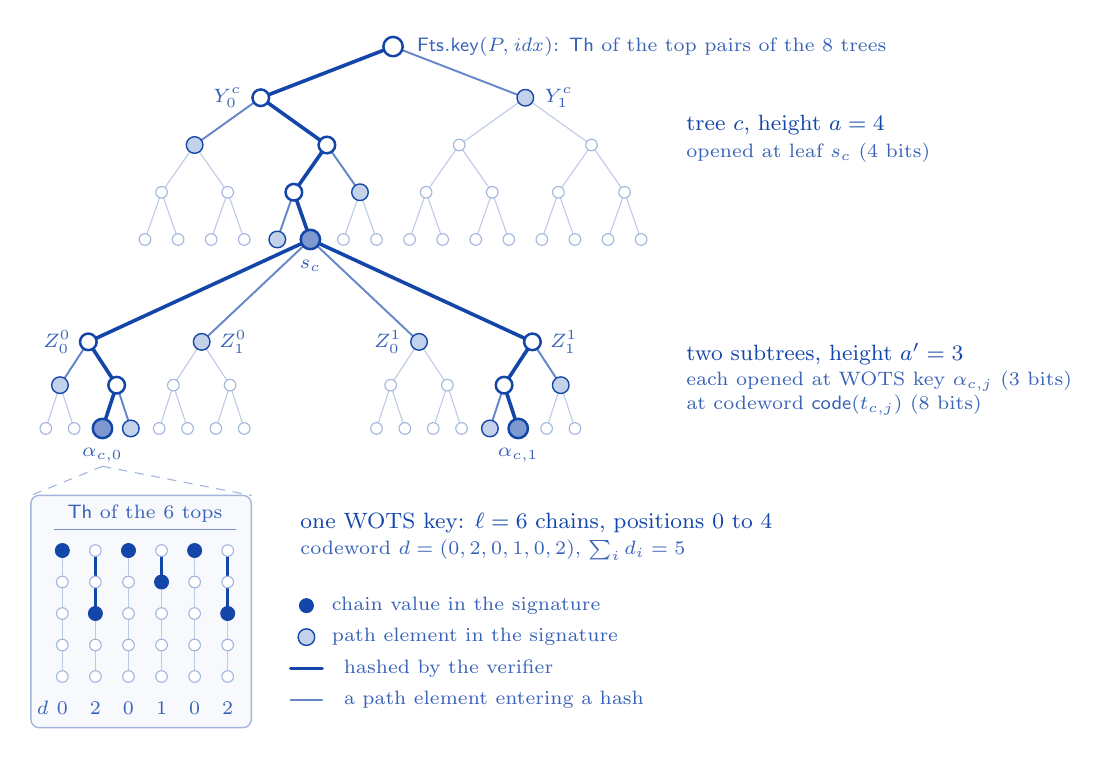
\begin{tikzpicture}[x=1cm,y=1cm,line join=round,line cap=round,
  tedge/.style={draw=fts!28,line width=0.4pt},
  input/.style={draw=fts!65,line width=0.7pt},
  path/.style={draw=fts,line width=1.3pt},
  plain/.style={circle,draw=fts!40,line width=0.4pt,fill=white,minimum size=4.2pt,inner sep=0pt},
  on/.style={circle,draw=fts,line width=0.9pt,fill=white,minimum size=6pt,inner sep=0pt},
  chosen/.style={circle,draw=fts,line width=0.9pt,fill=fts!55,minimum size=7pt,inner sep=0pt},
  auth/.style={circle,draw=fts,line width=0.5pt,fill=fts!25,minimum size=6pt,inner sep=0pt},
  rev/.style={circle,draw=fts,fill=fts,minimum size=5pt,inner sep=0pt},
  lab/.style={font=\footnotesize,text=fts},
  note/.style={font=\scriptsize,text=fts!85}]
% The tree: 16 leaves, three levels of nodes above them, no root.
\foreach \l in {1,2,3} {
  \pgfmathtruncatemacro{\last}{2^(4-\l)-1}
  \foreach \j in {0,...,\last} {
    \pgfmathsetmacro{\x}{((\j+0.5)*2^\l-8)*0.42}
    \pgfmathsetmacro{\xa}{((2*\j+0.5)*2^(\l-1)-8)*0.42}
    \pgfmathsetmacro{\xb}{((2*\j+1.5)*2^(\l-1)-8)*0.42}
    \draw[tedge] (\x,3+0.6*\l) -- (\xa,2.4+0.6*\l) (\x,3+0.6*\l) -- (\xb,2.4+0.6*\l);}}
\foreach \l in {0,...,3} {
  \pgfmathtruncatemacro{\last}{2^(4-\l)-1}
  \foreach \j in {0,...,\last} \node[plain] at ({((\j+0.5)*2^\l-8)*0.42},3+0.6*\l) {};}
% Its two subtrees, under leaf s_c = 5: 8 WOTS keys each, two levels above them.
\foreach \c in {-3.15,1.05} {
  \foreach \l in {1,2} {
    \pgfmathtruncatemacro{\last}{2^(3-\l)-1}
    \foreach \j in {0,...,\last} {
      \pgfmathsetmacro{\x}{\c+((\j+0.5)*2^\l-4)*0.36}
      \pgfmathsetmacro{\xa}{\c+((2*\j+0.5)*2^(\l-1)-4)*0.36}
      \pgfmathsetmacro{\xb}{\c+((2*\j+1.5)*2^(\l-1)-4)*0.36}
      \draw[tedge] (\x,0.6+0.55*\l) -- (\xa,0.05+0.55*\l) (\x,0.6+0.55*\l) -- (\xb,0.05+0.55*\l);}}
  \foreach \l in {0,1,2} {
    \pgfmathtruncatemacro{\last}{2^(3-\l)-1}
    \foreach \j in {0,...,\last} \node[plain] at ({\c+((\j+0.5)*2^\l-4)*0.36},0.6+0.55*\l) {};}}
% What the verifier is given and what it hashes: subtree 0 at key 2, subtree 1 at key 5.
\draw[input] (-3.33,0.6) -- (-3.51,1.15) (-4.23,1.15) -- (-3.87,1.7);
\draw[path] (-3.69,0.6) -- (-3.51,1.15) -- (-3.87,1.7);
\draw[input] (1.23,0.6) -- (1.41,1.15) (2.13,1.15) -- (1.77,1.7);
\draw[path] (1.59,0.6) -- (1.41,1.15) -- (1.77,1.7);
\draw[input] (-2.43,1.7) -- (-1.05,3) (0.33,1.7) -- (-1.05,3);
\draw[path] (-3.87,1.7) -- (-1.05,3) (1.77,1.7) -- (-1.05,3);
\draw[input] (-1.47,3) -- (-1.26,3.6) (-0.42,3.6) -- (-0.84,4.2) (-2.52,4.2) -- (-1.68,4.8);
\draw[path] (-1.05,3) -- (-1.26,3.6) -- (-0.84,4.2) -- (-1.68,4.8);
\draw[input] (1.68,4.8) -- (0,5.45);
\draw[path] (-1.68,4.8) -- (0,5.45);
\foreach \p in {(-3.33,0.6),(-4.23,1.15),(-2.43,1.7),(1.23,0.6),(2.13,1.15),(0.33,1.7),
  (-1.47,3),(-0.42,3.6),(-2.52,4.2),(1.68,4.8)} \node[auth] at \p {};
\foreach \p in {(-3.51,1.15),(-3.87,1.7),(1.41,1.15),(1.77,1.7),(-1.26,3.6),(-0.84,4.2),(-1.68,4.8)}
  \node[on] at \p {};
\foreach \p in {(-3.69,0.6),(1.59,0.6),(-1.05,3)} \node[chosen] at \p {};
\node[on,minimum size=7pt] at (0,5.45) {};
% Names of the nodes.
\node[note,anchor=east] at (-1.8,4.8) {$Y^c_0$};
\node[note,anchor=west] at (1.8,4.8) {$Y^c_1$};
\node[note,anchor=north] at (-1.05,2.86) {$s_c$};
\node[note,anchor=east] at (-3.97,1.7) {$Z^0_0$};
\node[note,anchor=west] at (-2.33,1.7) {$Z^0_1$};
\node[note,anchor=east] at (0.23,1.7) {$Z^1_0$};
\node[note,anchor=west] at (1.87,1.7) {$Z^1_1$};
\node[note,anchor=north] at (-3.69,0.47) {$\alpha_{c,0}$};
\node[note,anchor=north] at (1.59,0.47) {$\alpha_{c,1}$};
\node[note,anchor=west] at (0.18,5.45) {$\FtsKey(P,\idx)$: $\Th$ of the top pairs of the 8 trees};
\node[lab,anchor=west] at (3.6,4.45) {tree $c$, height $a=4$};
\node[note,anchor=west] at (3.6,4.1) {opened at leaf $s_c$ (4 bits)};
\node[lab,anchor=west] at (3.6,1.55) {two subtrees, height $a'=3$};
\node[note,anchor=west] at (3.6,1.2) {each opened at WOTS key $\alpha_{c,j}$ (3 bits)};
\node[note,anchor=west] at (3.6,0.9) {at codeword $\lut(t_{c,j})$ (8 bits)};
% One opened WOTS key, the codeword d = (0,2,0,1,0,2).
\draw[fts!40,line width=0.4pt,dashed] (-3.69,0.12) -- (-4.6,-0.25) (-3.69,0.12) -- (-1.8,-0.25);
\draw[fts!40,line width=0.5pt,rounded corners=3pt,fill=fts!3] (-4.6,-3.2) rectangle (-1.8,-0.25);
\node[note] at (-3.15,-0.48) {$\Th$ of the 6 tops};
\draw[fts!60,line width=0.4pt] (-4.3,-0.68) -- (-2.0,-0.68);
\foreach \i/\d in {0/0,1/2,2/0,3/1,4/0,5/2} {
  \pgfmathsetmacro{\x}{-4.2+0.42*\i}
  \pgfmathtruncatemacro{\r}{4-\d}
  \draw[tedge] (\x,-2.55) -- (\x,-0.95);
  \ifnum\d>0 \draw[path,line width=0.9pt] (\x,-2.55+0.4*\r) -- (\x,-0.95); \fi
  \foreach \q in {0,...,4} {\ifnum\q=\r \node[rev] at (\x,-2.55+0.4*\q) {};
    \else \node[plain] at (\x,-2.55+0.4*\q) {}; \fi}
  \node[note] at (\x,-2.95) {$\d$};}
\node[note] at (-4.45,-2.95) {$d$};
\node[lab,anchor=west] at (-1.3,-0.6) {one WOTS key: $\ell=6$ chains, positions $0$ to $4$};
\node[note,anchor=west] at (-1.3,-0.95) {codeword $d=(0,2,0,1,0,2)$, $\textstyle\sum_id_i=5$};
% Legend.
\node[rev] at (-1.1,-1.65) {}; \node[note,anchor=west] at (-0.9,-1.65) {chain value in the signature};
\node[auth] at (-1.1,-2.05) {}; \node[note,anchor=west] at (-0.9,-2.05) {path element in the signature};
\draw[path] (-1.3,-2.45) -- (-0.9,-2.45); \node[note,anchor=west] at (-0.75,-2.45) {hashed by the verifier};
\draw[input] (-1.3,-2.85) -- (-0.9,-2.85); \node[note,anchor=west] at (-0.75,-2.85) {a path element entering a hash};
\end{tikzpicture}
\caption{One of the $k=8$ trees of a forest, opened at the marks of a digest: leaf $s_c$, and in each subtree $j$ the WOTS key $\alpha_{c,j}$ at the codeword $\lut(t_{c,j})$. Neither the tree nor a subtree has a root: the verifier reaches one node of each top pair and reads the other in the signature.}
\label{fig:forest}
\end{figure}

A forest may sign several digests. Reuse leaks rather than breaks: a forgery at a forest needs, in every tree, the selected leaf's two selected WOTS keys already opened at codewords whose componentwise maximum covers the selected one.

\paragraph{Selecting the forest and its marks.}
\label{rem:rho}
For message $m$ and randomizer $\rho$, define
\[
  \Digest(P,m,\rho)=\hash(P\concat\addr_{\mathrm{msg}}\concat m\concat\rho).
\]
The root is not hashed: $P$ binds the key. The message ends the first block, so the second block is the randomizer alone, and the randomizer is $R_0+i$ rather than a hash: this is deliberate, so that every randomizer trial costs exactly one compression, the signer hashing the first block once. The digest's fields are grouped by kind, so that none lies across two 64-bit words. Its first 16 bytes are the codeword indices, a byte each:
\[
  t_{c,j}=\text{byte }2c+j.
\]
Interpret its last 16 bytes as a little-endian integer $N$, of which the low $h+4k+6k=106$ bits are used: the index, then the trees' leaves, then the subtrees' WOTS keys,
\[
  \idx=N\bmod2^h,\qquad
  s_c=\left\lfloor N/2^{h+4c}\right\rfloor\bmod2^4,\qquad
  \alpha_{c,j}=\left\lfloor N/2^{h+4k+3(2c+j)}\right\rfloor\bmod2^3,
  \quad j\in\{0,1\}.
\]
Every digest is accepted.

\section{The complete signature scheme}

\subsection{Key generation}
\label{rem:seed}

$\Gen(b)$ samples $S_0\getsr\bits{256}$, derives $S$ and $P$ as in Section~\ref{sec:parameters}, builds the kept subtree and the surrogates of Section~\ref{sec:pruning}, and folds them into $\rootnode$. It returns
\[
  \pk=(\rootnode,P),\qquad \sk=(S_0,b),
\]
the kept subtree being a cache the signer may recompute from $S_0$ and $b$.

\subsection{Signing}
\label{sec:sign}

Given $\sk=(S_0,b)$ and a 256-bit message $m$, $\Sig(\sk,m)$ proceeds as follows:
\begin{enumerate}
\item Derive $R_0=\Th(P,\addr_{\mathrm{rnd}},S\concat m)$. For $i=0,\ldots,\amax-1$, let $\rho_i=R_0+i$ as 128-bit little-endian integers, modulo $2^{128}$. Stop at the first $i$ for which the index of $\Digest(P,m,\rho_i)$ is a kept leaf, set $\rho=\rho_i$, and extract $\idx$ and the marks. Return $\bot$ if no trial succeeds. A full key stops at $i=0$.
\item Compute the opening $\FtsOpen(P,\idx,\text{marks})$ and $M=\FtsKey(P,\idx)$.
\item Compute $(c,\sigma)=\OtsSign(P,\idx,M)$, returning $\bot$ on failure, and the authentication path $A$ of leaf $\idx$.
\item Return the randomizer, the opening, $c$, $\sigma$ and $A$.
\end{enumerate}
Signing is deterministic and changes no secret state. Repeating a message returns the same signature, or the same failure.

\subsection{Verification}
\label{sec:ver}

$\Ver(\pk,m,\sigma)$ rejects $\bot$ and malformed inputs. Otherwise, parse $\pk=(\rootnode,P)$ and $\sigma$ as above:
\begin{enumerate}
\item Compute $\Digest(P,m,\rho)$ and extract $\idx$ and the marks.
\item Set $M=\FtsRec(P,\idx,\text{marks},\text{opening})$.
\item Compute $X=\OtsLeaf(P,\idx,M,c,\sigma)$. Reject if $X=\bot$.
\item Accept exactly when $\TreeFold(P,\idx,X,A)=\rootnode$.
\end{enumerate}

\subsection{Serialization and cost}
\label{sec:costs}

Serialize the public key as $\rootnode\concat P$, 32 bytes. The secret key is $S_0\concat\LE_8(b)$, 33 bytes: $b$ places the kept subtree and its surrogates, and so the root.

A signature starts with $\rho$, followed by the forest's opening in increasing tree, then $\LE_{32}(c)$, the $v$ chain values in increasing chain index, and the path in increasing height. A tree's opening is, for each of its two subtrees, the six chain values in increasing chain index then the three siblings in increasing height, followed by the tree's four siblings. The size is
\[
  \underbrace{16}_{\rho}
  +\underbrace{k\,(2(\ell+a')+a)\,16}_{\text{forest opening}}
  +\underbrace{4+v\,16}_{\text{WOTS$^+$C}}
  +\underbrace{h\,16}_{\text{path}}
  =4276\text{ bytes}.
\]

Count compressions of BLAKE2s: an input of $r$ bytes costs $\lceil r/64\rceil$. Every signature takes exactly
\[
  \underbrace{2}_{\text{digest}}
  +\underbrace{k\bigl(2(5+2+2)+2+3\bigr)+5}_{\text{forest}}
  +\underbrace{1+(2^w-1)v-T+17}_{\text{WOTS$^+$C}}
  +\underbrace{h}_{\text{path}}
  =307
\]
compressions to verify: per subtree 5 chain steps, 2 for the WOTS key's leaf and 2 folds, then 2 for the tree leaf and 3 folds, and 5 for the public key of the forest.

A one-time key takes $32$ derivations and $192$ chain steps, so its leaf $241$ compressions and key generation $242\cdot2^b+2(h-b)+1$. A forest holds $2048$ WOTS keys of $29$ compressions each, which is what signing spends its hashes on: about $6\cdot10^4$, plus the $2^{h-b}$ expected randomizer trials of a pruned key, one compression each, and the expected $829$ encoding attempts.

\section{Security}
\label{sec:security}

Model $\hash$ as one shared random oracle. The challenger generates a key pair and gives $\pk$ to a classical probabilistic adversary, which may adaptively query the hash and request signatures on messages of its choice, at most $N$ of them. It finally returns $(m^*,\sigma^*)$ and wins exactly when $\Ver(\pk,m^*,\sigma^*)=1$ and no signing request for $m^*$ returned $\sigma^*$: \emph{strong unforgeability}. A query budget $q$ bounds every hash call of the complete experiment, including key generation, signing and final verification.

The lifetime $N$ of a key depends on the height $b$ of the subtree it keeps. For each row below, with $N$ rounded down, every adversary making at most $N$ signing requests wins with probability at most $q/2^{127}$. Key generation costs $242\cdot2^b+2(h-b)+1$ compressions (Section~\ref{sec:costs}), rounded to nearest:
\begin{center}
\begin{tabular}{@{}rrr@{}}
\toprule
$b$ & lifetime $N$ (signatures) & key generation (compressions)\\
\midrule
26 & 1.3B & 16B\\
20 & 26M & 250M\\
14 & 480K & 4.0M\\
13 & 240K & 2.0M\\
12 & 120K & 990K\\
10 & 33K & 250K\\
8 & 8.8K & 62K\\
\bottomrule
\end{tabular}
\end{center}
These lifetimes are proved in Lean~4, with only Lean's three standard axioms, in \texttt{formal/lean\_sphincs/} (\texttt{Sphincs.Lifetimes.requestedSecurity}), for the scheme of this document: its hash inputs, its codeword table and its signer.

\paragraph{Layout.}
\label{sec:layout}
The bytes of two things are chosen so that a prover whose machine words are 16 bytes never cuts a value in two and never reads a field across two 64-bit words. The address is 8 bytes of fields followed by 8 zero bytes; with it the message ends the digest's first block. And the digest's fields are grouped by kind rather than by tree.

\paragraph{Hash domains.}
An input determines its parameter, its address and its payload, and an address determines the call, so distinct calls of one key never share an input. Calls of different keys differ in $P$.

\paragraph{Quantum security.}
\label{sec:quantum}
Approximately 64 bits of security in the quantum random-oracle model is a target. No quantum security bound is proved here.

\section{Completeness}
\label{sec:completeness}

Signing fails only if the randomizer search or the counter search is exhausted; whenever it succeeds, verification accepts, each recovery retracing what the signer computed.

A randomizer trial selects a kept leaf with probability $2^{-(h-b)}$, so for $b\geq8$ the search fails with probability about $(1-2^{-18})^{\amax}\leq e^{-2^{14}}$. An encoding accepts exactly when its 64 two-bit positions sum to 120, so a uniform 128-bit digest is accepted with probability
\[
  \frac{[z^{120}](1+z+z^2+z^3)^{64}}{2^{128}}
  =\frac{410356077965267834847013187094862224}{2^{128}}
  \geq2^{-10},
\]
where $[z^r]$ denotes the coefficient of $z^r$, and all $\cmax=2^{32}$ counters fail with probability at most $e^{-2^{22}}$.

\appendix
\section{Address encoding}
\label{sec:tweaks}

An address is 16 bytes: a 32-bit field $\mathit{lo}$, a 24-bit field $\mathit{hi}$, one byte holding a 5-bit type $t$ and a 3-bit chain step $\mu$, and 8 zero bytes,
\[
  \mathsf{enc}(t,\mu,\mathit{hi},\mathit{lo})=\LE_{32}(\mathit{lo})\concat\LE_{24}(\mathit{hi})\concat\LE_8(t+32\mu)\concat0^{64}.
\]
In the tree, $\mathit{lo}$ is a leaf or a node index. In a forest, $\mathit{lo}$ is $\idx$ and $\mathit{hi}$ packs the position: write $\pi=c+8s+128j$ for a subtree and $\pi+256\alpha$ for a WOTS key.

\begin{center}
\small
\begin{tabular}{@{}ll@{}}
\toprule
Address & Encoding\\
\midrule
$\addr_{\mathrm{prf}}(e,r)$ & $\mathsf{enc}(0,0,r,e)$\\
$\addr_{\mathrm{chain}}(e,i,\mu)$ & $\mathsf{enc}(1,\mu,i,e)$\\
$\addr_{\mathrm{leaf}}(e)$ & $\mathsf{enc}(2,0,0,e)$\\
$\addr_{\mathrm{node}}(\lambda,j)$ & $\mathsf{enc}(3,0,\lambda,j)$\\
$\addr_{\mathrm{enc}}(e)$ & $\mathsf{enc}(4,0,0,e)$\\
$\addr_{\mathrm{parameter}}$ & $\mathsf{enc}(5,0,0,0)$\\
$\addr_{\mathrm{rnd}}$ & $\mathsf{enc}(7,0,0,0)$\\
$\addr_{\mathrm{msg}}$ & $\mathsf{enc}(12,0,0,0)$\\
$\addr_{\mathrm{surrogate}}(\lambda)$ & $\mathsf{enc}(13,0,\lambda,0)$\\
$\addr_{\mathrm{fprf}}(\idx,c,s,j,\alpha,r)$ & $\mathsf{enc}(14,0,\pi+256\alpha+2048r,\idx)$\\
$\addr_{\mathrm{fchain}}(\idx,c,s,j,\alpha,i,\mu)$ & $\mathsf{enc}(15,\mu,\pi+256\alpha+2048i,\idx)$\\
$\addr_{\mathrm{fkey}}(\idx,c,s,j,\alpha)$ & $\mathsf{enc}(16,0,\pi+256\alpha,\idx)$\\
$\addr_{\mathrm{fsub}}(\idx,c,s,j,\lambda,\nu)$ & $\mathsf{enc}(17,0,\pi+256\lambda+1024\nu,\idx)$\\
$\addr_{\mathrm{fleaf}}(\idx,c,s)$ & $\mathsf{enc}(18,0,c+8s,\idx)$\\
$\addr_{\mathrm{fnode}}(\idx,c,\lambda,\nu)$ & $\mathsf{enc}(19,0,c+8\lambda+64\nu,\idx)$\\
$\addr_{\mathrm{froots}}(\idx)$ & $\mathsf{enc}(20,0,0,\idx)$\\
\bottomrule
\end{tabular}
\end{center}

In a chain address, $\mu$ is the position the step leaves. Types $0$, $5$, $7$, $13$ and $14$ are reserved for the signer's derivations from the seed.

\section{The codeword table}
\label{sec:codewords}

Sort the 246 codewords by decreasing $\sum_id_i^2$, and codewords with equal sums lexicographically, $d_0$ first. Then $\lut(t)$ is codeword number $t\bmod214$ of that list. The table thus leaves out the 32 most spread-out codewords and holds the 42 most concentrated twice: spread-out codewords are the easier to cover once a key has signed twice.
\begin{center}
\begin{tabular}{@{}lrrr@{}}
\toprule
Digits of the codeword & $\sum_id_i^2$ & codewords & entries\\
\midrule
$\{4,1\}$ & 17 & 30 & 60\\
$\{3,2\}$ & 13 & 30 & 42\\
$\{3,1,1\}$ & 11 & 60 & 60\\
$\{2,2,1\}$ & 9 & 60 & 60\\
$\{2,1,1,1\}$ & 7 & 60 & 34\\
$\{1,1,1,1,1\}$ & 5 & 6 & 0\\
\bottomrule
\end{tabular}
\end{center}

\bibliographystyle{alphaurl}
\bibliography{refs}

\end{document}
